%%%%%%%%%%%%%%%%%%%%%%%%%%%%%%%%
%%% 課題I
%%%%%%%%%%%%%%%%%%%%%%%%%%%%%%%%

\homework

%%%%%%%%%%%%%%%%%%%%%%%%%%%%%%%%
%%% I-1
%%%%%%%%%%%%%%%%%%%%%%%%%%%%%%%%

\question{
	\textsf{プログラミングツールのツール:}
	BCCにはMAKEユーティリティの他,grepやtouchなどプログラム開発に行う際に役に立つ
	コマンドラインツールが含まれている.それぞれの機能や利用法について学習せよ.\\
}

\vspace{-\baselineskip}

% make

\subquestion{MAKEユーティリティ}

Makeは,プログラムのビルドを自動化するために用いられるツールである.
ビルド作業が複雑になるときに特に役に立つ.
例えば,複雑に関連したソースファイルなどをビルドするとき,
長いコマンドや複数のコマンドが必要になる.
Makeによりそれらを一つにまとめビルド作業を簡単化できる.
makeコマンドを使うためにMakefileを規則に従って作る必要がある.
コマンドは以下のように使用する.\cite{Make}

\begin{lstlisting}[tabsize=1, numberstyle=\color{white}]
	make target
\end{lstlisting}

\vspace{-\baselineskip}

% Grep

\subquestion{grep}

Grepはテキストファイルから指定されたパターン(文字列)を1つまたは複数検索する.
コマンドを使うときにオプションを指定することでアルファベットの大文字小文字の区別
などを設定できる.コマンドは以下のように使用する.\cite{Grep}

\begin{lstlisting}[tabsize=1, numberstyle=\color{white}]
	grep [option] pattern file
\end{lstlisting}

\vspace{-\baselineskip}

% touch

\subquestion{touch}

touchは指定したファイルのアクセス時間(atime)や修正時間(mtime)を
書き換える.作成時間(ctime)は書き換えない.
コマンドは以下のように使用する.\cite{touch}

\begin{lstlisting}[tabsize=1, numberstyle=\color{white}]
	touch [option] file
\end{lstlisting}

%%%%%%%%%%%%%%%%%%%%%%%%%%%%%%%%
%%% I-2
%%%%%%%%%%%%%%%%%%%%%%%%%%%%%%%%

\question{
	\textsf{C言語:}変数の「有効範囲(Scope)」,「記憶域期間(記憶寿命)」
	について学習し,一般的な(ローカル)変数とグローバル変数,
	スタティック変数の違いを整理せよ.\\
}

\vspace{-\baselineskip}

% 有効範囲(Scope)

\subquestion{有効範囲(Scope)}

「有効範囲(Scope)」には,ブロック内を有効範囲(ブロック有効範囲)とする場合と
ファイル内を有効範囲(ファイル有効範囲)とする場合がある.
ブロック内とは\texttt{\{\}}で囲まれた部分のことで,
ファイル内とはファイル全ての範囲のことである.\cite{isl}

% 記憶域期間(記憶寿命)

\subquestion{記憶域期間(記憶寿命)}

「記憶域期間(記憶寿命)」には,自動記憶域期間と静的記憶域期間がある.
自動記憶域期間とは\texttt{auto}
\footnote{\texttt{auto}は省略することができるので一般に明示はしない.}
を使用して宣言したオブジェクト(変数)が持つ記憶域期間のことで,
オブジェクトは宣言したブロックに入ったときから終了するまで生存する.
静的記憶域期間とは,ファイル有効範囲のオブジェクトか\texttt{static}
を使用して宣言したときにオブジェクトが持つ記憶域期間のことで,
プログラムの開始から終了するまで生存する.\cite{atmarkit}

\pagebreak

\subquestion{各変数の有効範囲と記憶域期間}

ローカル変数,グローバル変数,スタティック変数の
有効範囲と記憶域期間をまとめたものを\Tblref{tbl:variable}に示す.
\begin{table}[htb]
	\centering
	\caption{各変数の有効範囲と記憶域期間}
	\begin{tabular}{l|c|c} \hline\hline
		\multicolumn{1}{c|}{変数} & 有効範囲 & 記憶域期間 \\ \hline
		ローカル変数     & ブロック有効範囲 & 自動記憶域期間 \\
		グローバル変数   & ファイル有効範囲 & 静的記憶域期間 \\
		スタティック変数 & ブロック有効範囲 & 静的記憶域期間 \\ \hline
	\end{tabular}
	\label{tbl:variable}
\end{table}

%%%%%%%%%%%%%%%%%%%%%%%%%%%%%%%%
%%% I-3
%%%%%%%%%%%%%%%%%%%%%%%%%%%%%%%%

\question{
	テキストの図1,図2のような図形(星型正多角形)を描き,
	回転させるプログラムを作成せよ.\\
}

\vspace{-\baselineskip}

% 星型正多角形

\subquestion{星型正多角形}

星型正多角形とは,正多角形と同様に全ての辺の長さが等しく全ての内角の大きさが等しいが
正多角形とは異なり辺同士が交わり合っている図形である.
注意として六芒星\footnote{2つの正三角形が重なってできている図形.}
のような幾つかの正多角形に分解できるものは星型正多角形に含まれない.
つまり,星型正多角形は一筆書きで書くことができる.\cite{Star}

$n$本の辺からなり元の位置に戻るために$m$周する星型正多角形について
$m$は多角形の密度と呼ばれ,星型正多角形になるための条件は,
$n$と$m$の最大公約数が$1$かつ,$n > 2m$である.
外角の和は$m$周することから$2\pi m$となり,
外角は$2\pi m / n = 2\pi / (n/m)$
\footnote{正多角形の場合も$m=1$となることから,この式は使える.}
で求めることができる.
このことから正多角形を星型正多角形に拡張して,正$n/m$角形と呼ばれる.
また,シュレーフリ記号(Schläfli symbol)では$\{n/m\}$と表記される.

% プログラム

\subquestion{プログラム}

演習3で作成した正多角形を描画するプログラムを
書き換えて星型正多角形(正$n/m$角形)を描画するプログラムを作成する.
作成した星型正多角形を描画する関数(\texttt{dispStarPolygon})を
\Lstref{lst:hw1-3-1}に示す.この関数は順に$n$,$m$,$\theta$を引数としている.
$\theta$は基準となる角度で,値を変えることで星型正多角形を回転させることができる.
関数\texttt{dispStarPolygon}を使い正$n/m$角形を回転させるためのプログラムを
\Lstref{lst:hw1-3-2}に示す.
\Lstref{lst:hw1-3-2}は1,2行目で正7/3角形に設定していて,
テキストのリスト11のタイマーコルバック関数を用いて,
$100\;[\mathrm{ms}]$経つたびに\texttt{rotAng}を$\pi/180$増加させ回転させている.
このプログラムの出力結果を\Figref{fig:hw1-3}に示す.

\lstinputlisting[
	caption = 星型正多角形を描画する関数(\texttt{dispStarPolygon}),
	label = lst:hw1-3-1,
	linerange = {28-31, 33-33, 35-43}
]{
	../../Homework/1/hw1-3.c
}
\lstinputlisting[
	caption = 星型正多角形を回転させるプログラム(主要部),
	label = lst:hw1-3-2,
	linerange = {5-6, 13-16, 18-18, 20-21, 23-23, 25-26}
]{
	../../Homework/1/hw1-3.c
}

%%%%%%%%%%%%%%%%%%%%%%%%%%%%%%%%
%%% I-4
%%%%%%%%%%%%%%%%%%%%%%%%%%%%%%%%

\question{
	テキストの図3,図4のような図形(完全グラフ)を描き,
	回転させるプログラムを作成せよ.\\
}

\vspace{-\baselineskip}

% 完全グラフ

\subquestion{完全グラフ}

完全グラフとは任意の2頂点間に必ずグラフがあるグラフのことをいう.
頂点が$n$個の完全グラフを$K_{n}$と表記し,
辺の数は頂点の組み合わせの数になるので$n(n-1) / 2$となる.\cite{Complete}

% プログラム

\subquestion{プログラム}

頂点の数が$n$の完全グラフ($K_{n}$)を描画するプログラムを作成する.
作成した完全グラフを描画する関数(\texttt{dispCompleteGraph})を
\Lstref{lst:hw1-4-1}に示す.この関数は順に$n$,$\theta$を引数としている.
まず全ての頂点の座標を配列に格納し,その後全ての辺を描いている.
関数\texttt{dispCompleteGraph}を使い$K_{n}$を回転させるためのプログラムは
\Lstref{lst:hw1-3-2}の9行目の\Lstref{lst:hw1-4-2}に書き換えたものとなる.
$n = 7$としたとき出力結果を\Figref{fig:hw1-4}に示す.

\lstinputlisting[
	caption = 完全グラフを描画する関数(\texttt{dispCompleteGraph}),
	label = lst:hw1-4-1,
	linerange = {27-31, 33-39, 41-52}
]{
	../../Homework/1/hw1-4.c
}
\lstinputlisting[
	caption = 関数\texttt{dispCompleteGraph}の呼び出し部分,
	label = lst:hw1-4-2,
	linerange = {20-20}
]{
	../../Homework/1/hw1-4.c
}

% 3, 4の出力結果

\begin{figure}[htbp]
	\centering
	\begin{minipage}[b]{0.45\textwidth}
		\centering
		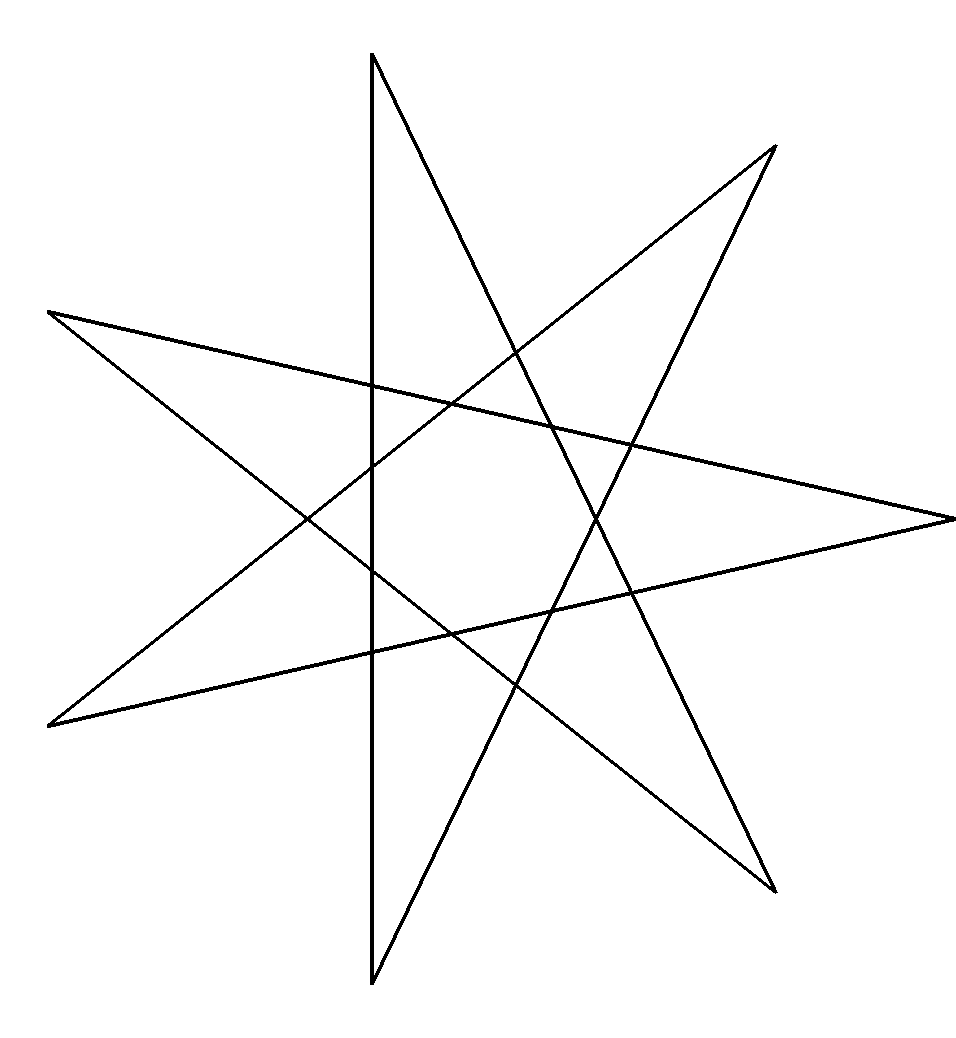
\includegraphics[scale=0.1]{../../Homework/1/data/hw1-3.png}
		\caption{正$7/3$角形の出力結果}
		\label{fig:hw1-3}
	\end{minipage}
	\begin{minipage}[b]{0.45\textwidth}
		\centering
		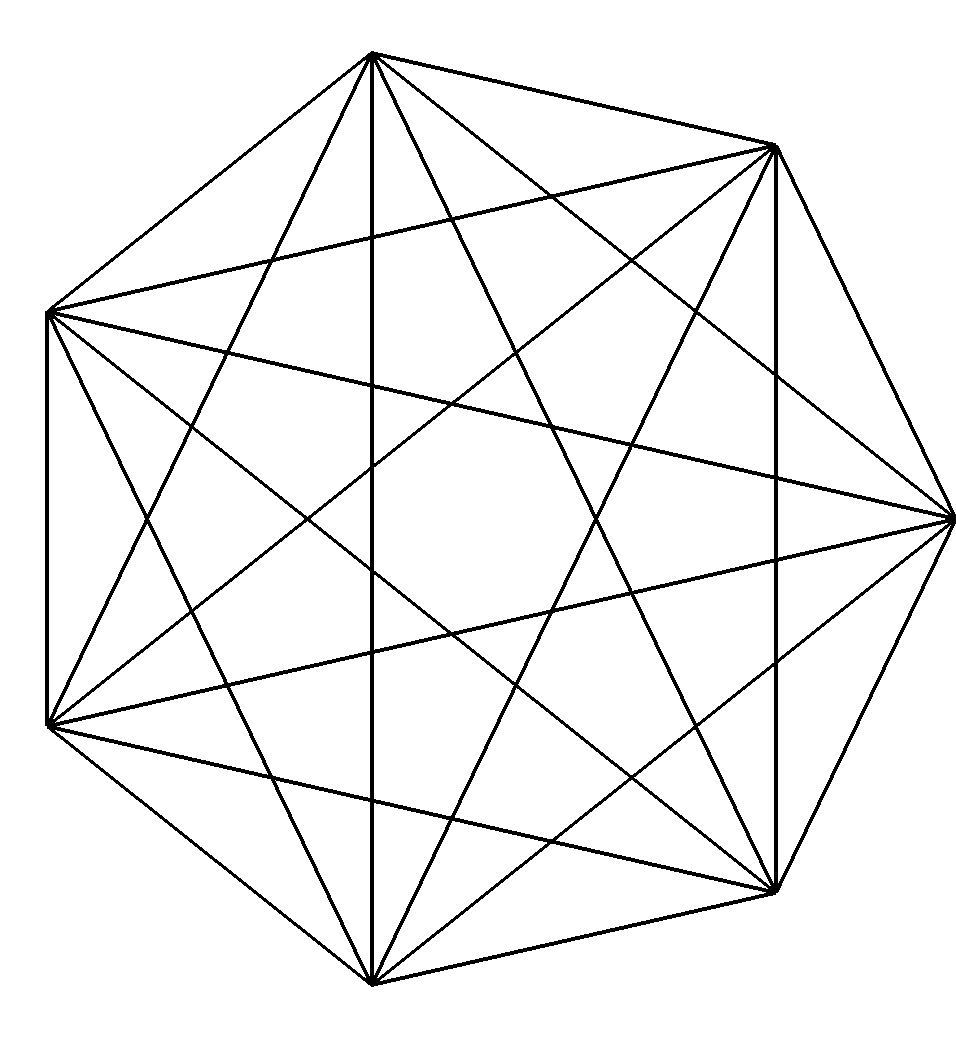
\includegraphics[scale=0.1]{../../Homework/1/data/hw1-4.png}
		\caption{$K_{7}$の出力結果}
		\label{fig:hw1-4}
	\end{minipage}
\end{figure}

%%%%%%%%%%%%%%%%%%%%%%%%%%%%%%%%
%%% I-5
%%%%%%%%%%%%%%%%%%%%%%%%%%%%%%%%

\question{
	テキストのリスト12を解析し,数学関数のグラフを描くプログラムを作成せよ.
	例えば$\theta$を$0$から$2\pi$まで変化させながら,次の関数をプロットすると
	どんな図形が描かれるだろうか(コラム参照).
	余力がある学生は,座標軸に目盛り(文字)を加えてみよ.
}

\begin{enumerate}
	\item カージオイド(cardioid)
	\begin{align}
		x &= [1 + \cos(\theta)]\cos(\theta)\label{equ:cardi-x}\\
		y &= [1 + \cos(\theta)]\sin(\theta)\label{equ:cardi-y}
	\end{align}
	\item サイクロイド(cycloid)
	\begin{align}
		x &= \theta - \sin(\theta)\label{equ:cycl-x}\\
		y &= 1 - \cos(\theta)\label{equ:cycl-y}
	\end{align}
	\item 4尖点の内サイクロイド(hypocycloid)
	\begin{align}
		x &= \cos^{3}(\theta)\label{equ:hypocycl-x}\\
		y &= \sin^{3}(\theta)\label{equ:hypocycl-y}
	\end{align}
\end{enumerate}

% プログラム

\subquestion{プログラム}

\Lstref{lst:hw1-5-1}にグラフを描画するために作成した関数のプロトタイプ宣言を示す.
関数\texttt{funcX},\texttt{funcY}に描くグラフの関数を設定する.
関数\texttt{setRange},\texttt{setXtics},\texttt{setYtics},\texttt{setRatio}は
グラフの設定パラメータを格納しているグローバル変数の書き換えをする関数で,
2つの軸の範囲,$x$軸の目盛り,$y$軸の目盛り,グラフの縦横比を設定する.
関数\texttt{dispGraph}はグラフを描くための関数で,関数内に目盛りを描くための
関数\texttt{drawXtics},\texttt{drawYtics}を使用する.
関数\texttt{dispGraph}を\Lstref{lst:hw1-5-2}に示す.
5から20行目でグラフの軸と目盛りを描画し,
22から28行目でグラフを描画している.
関数\texttt{setXtics},\texttt{setYtics}を\Lstref{lst:hw1-5-x},\Lstref{lst:hw1-5-y}に示す.
これらの関数はどちらも7から15行で$2l$の長さの目盛りを引いている.
17から29行目で,\texttt{setXtics}は表示する数字を目盛りの下になるようにして
\texttt{setYtics}は表示する数字を目盛りの左になるようにしている.

\lstinputlisting[
	caption = 関数のプロトタイプ宣言部分,
	label = lst:hw1-5-1,
	linerange = {9-17}
]{
	../../Homework/1/hw1-5.c
}
\lstinputlisting[
	caption = グラフ描画関数(\texttt{dispGraph}),
	label = lst:hw1-5-2,
	linerange = {32-60}
]{
	../../Homework/1/hw1-5.c
}
\lstinputlisting[
	caption = $x$軸の目盛り描画関数(\texttt{drawXtics}),
	label = lst:hw1-5-x,
	linerange = {62-91}
]{
	../../Homework/1/hw1-5.c
}
\lstinputlisting[
	caption = $y$軸の目盛り描画関数(\texttt{drawYtics}),
	label = lst:hw1-5-y,
	linerange = {93-122}
]{
	../../Homework/1/hw1-5.c
}

% 出力

\subquestion{各関数の出力結果}

この関数でカージオイド,サイクロイド,4尖点の内サイクロイドを
適切に軸の範囲や目盛りを設定して描画したグラフを
\Figref{fig:hw1-5-a},\Figref{fig:hw1-5-b},\Figref{fig:hw1-5-c}に示す.

\begin{figure}[htbp]
	\centering
	\begin{minipage}[b]{0.32\textwidth}
		\centering
		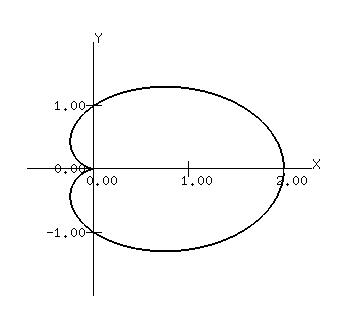
\includegraphics[scale=0.39]{../../Homework/1/data/hw1-5-a.png}
		\caption{カージオイド}
		\label{fig:hw1-5-a}
	\end{minipage}
	\begin{minipage}[b]{0.32\textwidth}
		\centering
		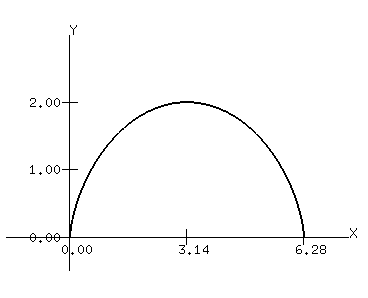
\includegraphics[scale=0.39]{../../Homework/1/data/hw1-5-b.png}
		\caption{サイクロイド}
		\label{fig:hw1-5-b}
	\end{minipage}
	\begin{minipage}[b]{0.32\textwidth}
		\centering
		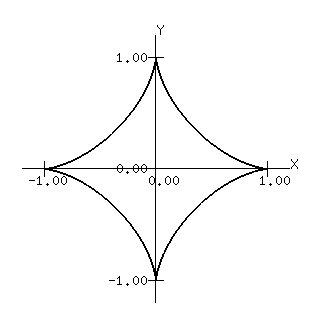
\includegraphics[scale=0.39]{../../Homework/1/data/hw1-5-c.png}
		\caption{4尖点の内サイクロイド}
		\label{fig:hw1-5-c}
	\end{minipage}
\end{figure}
